\documentclass{article}
\usepackage[UTF8]{ctex}
% Replace `letterpaper' with`a4paper' for UK/EU standard size
\usepackage[a4paper,top=2cm,bottom=2cm,left=3cm,right=3cm,marginparwidth=1.75cm]{geometry}

% Useful packages
\usepackage{amsmath}
\usepackage{mathrsfs,amsmath}
\usepackage{graphicx}
\usepackage[colorlinks=true, allcolors=blue]{hyperref}
\usepackage{graphicx} %插入图片的宏包
\usepackage{float} %设置图片浮动位置的宏包
\usepackage{subfigure} %插入多图时用子图显示的宏包
\usepackage{parskip}
\usepackage{indentfirst} 
\setlength{\parindent}{2em}
\usepackage{hyperref}  
\usepackage{tikz}
\allowdisplaybreaks
\usepackage{multirow}
\usepackage{amsmath}
\usepackage{amsfonts,amssymb} 
\usepackage{xcolor} % 用于显示颜色
\usepackage{listings} % 用于插入代码
\lstset{
	basicstyle          =   \sffamily,          % 基本代码风格
	keywordstyle        =   \bfseries,          % 关键字风格
	commentstyle        =   \rmfamily\itshape,  % 注释的风格,斜体
	stringstyle         =   \ttfamily,  % 字符串风格
	flexiblecolumns,                % 别问为什么,加上这个
	numbers             =   left,   % 行号的位置在左边
	showspaces          =   false,  % 是否显示空格,显示了有点乱,所以不现实了
	numberstyle         =   \zihao{-5}\ttfamily,    % 行号的样式,小五号,tt等宽字体
	showstringspaces    =   false,
	captionpos          =   t,      % 这段代码的名字所呈现的位置,t指的是top上面
	frame               =   lrtb,   % 显示边框
}

\lstdefinestyle{Python}{
	language        =   Python, % 语言选Python
	basicstyle      =   \zihao{-5}\ttfamily,
	numberstyle     =   \zihao{-5}\ttfamily,
	keywordstyle    =   \color{blue},
	keywordstyle    =   [2] \color{teal},
	stringstyle     =   \color{magenta},
	commentstyle    =   \color{red}\ttfamily,
	breaklines      =   true,   % 自动换行,建议不要写太长的行
	columns         =   fixed,  % 如果不加这一句,字间距就不固定,很丑,必须加
	basewidth       =   0.5em,
}

\title{图像处理与可视化Homework3 报告}
\author{林子开 21307110161}
\begin{document}
	\maketitle
	\tableofcontents

\section{Implementation of Spatial Filter}
\subsection{Smoothing}
\subsubsection{Introduction to My Algorithm and the Python Codes}
I've completed the smoothing algorithm in two methods. The first is to
take the \textbf{local average} of the kernel and the second is 
to make convolution with a \textbf{Gauss kernel}. 

User may set different kernel size for the first method, e.g., $3\times 3$,
and the corresponding efficient, e.g., $\frac{1}{9}$, will be computed automatically.
As for the Gauss kernel method, user need to set $\sigma$. The algorithm assumes the 
density function of Gauss distribution beyond $3\sigma$ is just 0 and will automatically
calculate the kernel size.

In addition, my algorithm will pad the original figure with pixels of intensity 127 before
smoothing, in order to maintain the size of smoothed figures as the original one. 

Here are the Pythond codes of my smoothing algorithm. Note that I've imported
\textbf{numba} to speed up my algorithm. Please install it first.

\lstinputlisting[style = Python,
caption={Python codes of my smoothing algorithm},
label = {smooth}]{exercise1_平滑.py}

\subsubsection{Experiment Results}
The original figure is as follows:
\begin{figure}[H]
	\centering
	{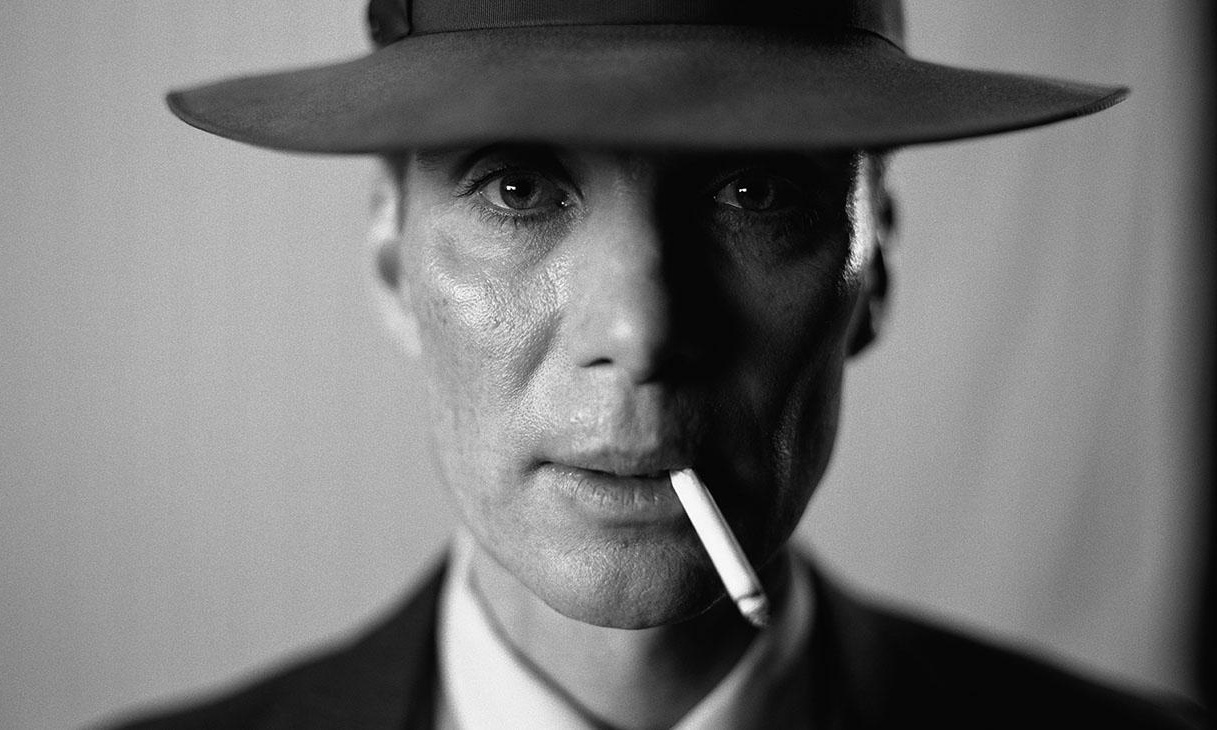
\includegraphics[width=0.45\textwidth]{test.jpeg}} 
	\caption{the original figure} \label{testFig}
\end{figure}

The smoothed figures by the local average method are like:
\begin{figure}[H]
    \centering
    \subfigure[kernel size = 3]
    {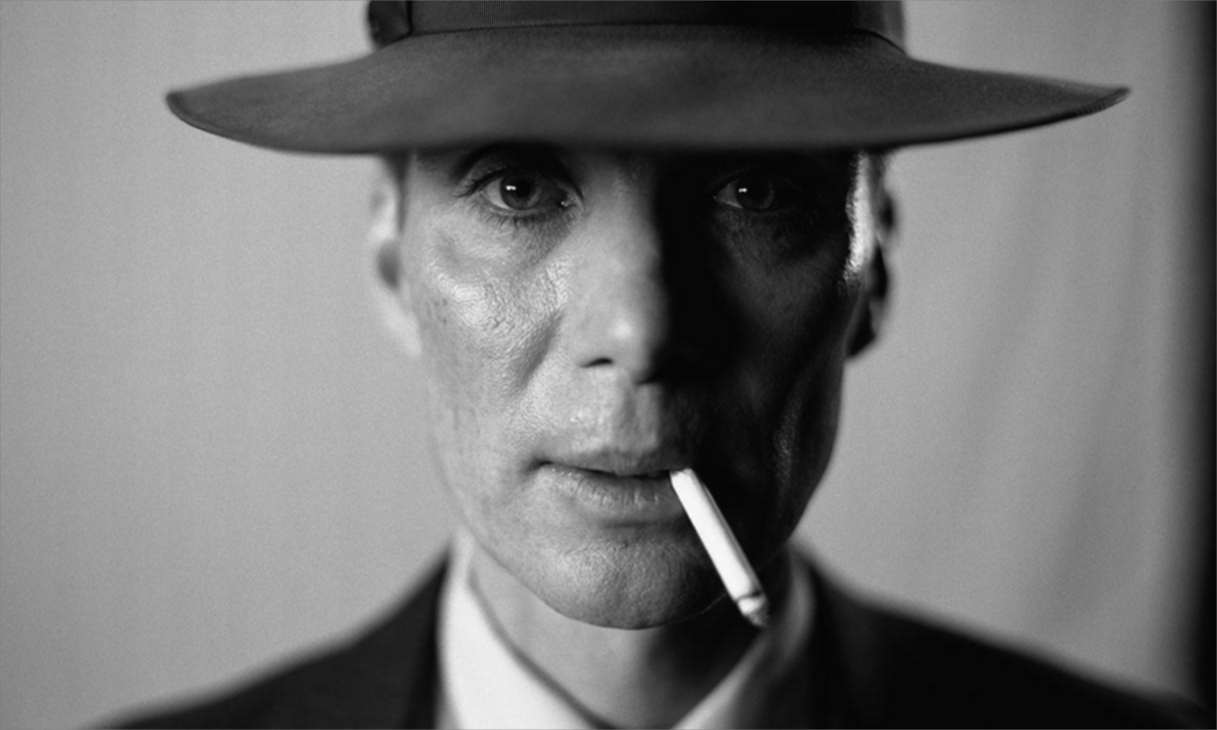
\includegraphics[width=0.45\textwidth]{result1//smooth_average_kernelSize=3.png}}
    \,    
    \subfigure[kernel size = 5]
    {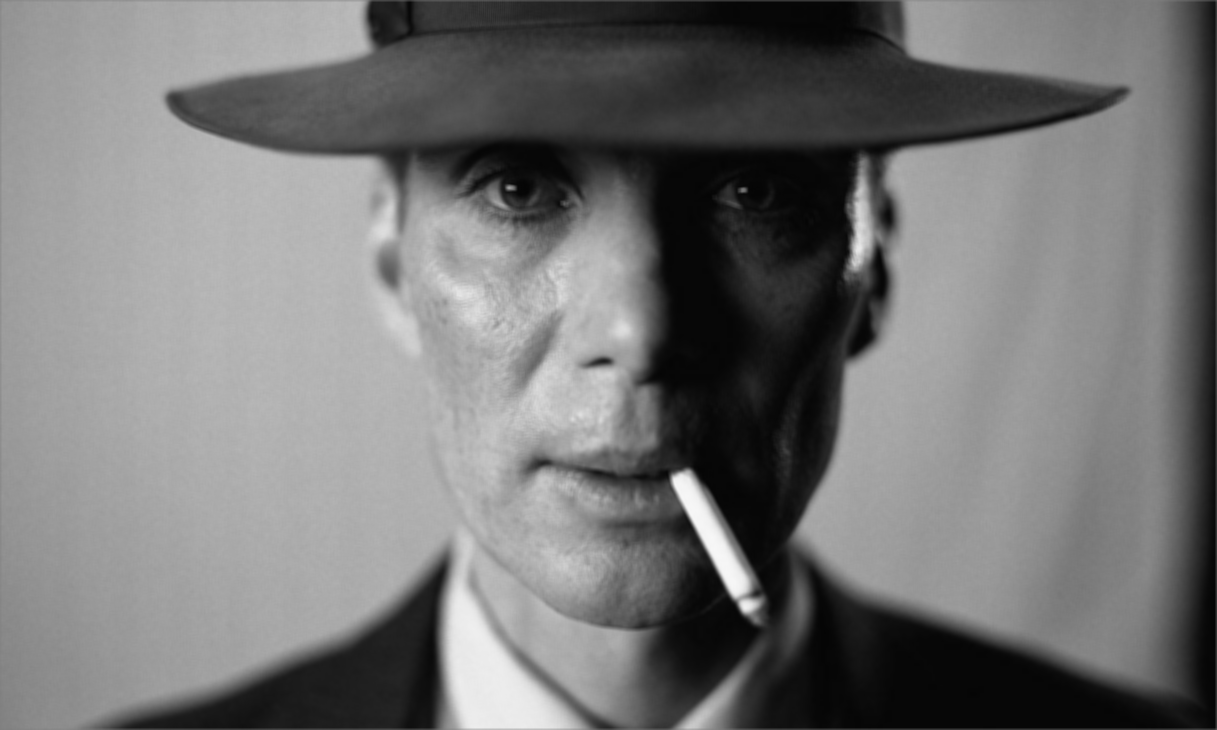
\includegraphics[width=0.45\textwidth]{result1//smooth_average_kernelSize=5.png}}
    \,
    \subfigure[kernel size = 7]
    {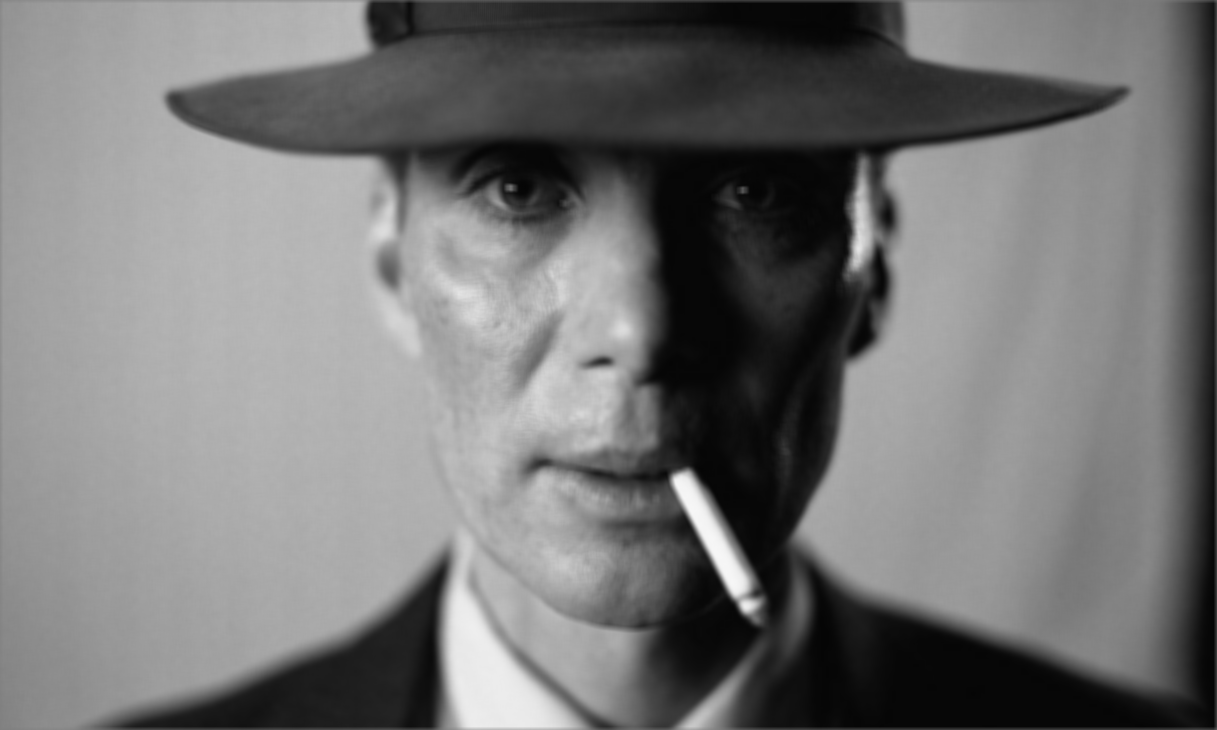
\includegraphics[width=0.45\textwidth]{result1//smooth_average_kernelSize=7.png}}
    \,    
    \subfigure[kernel size = 9]
    {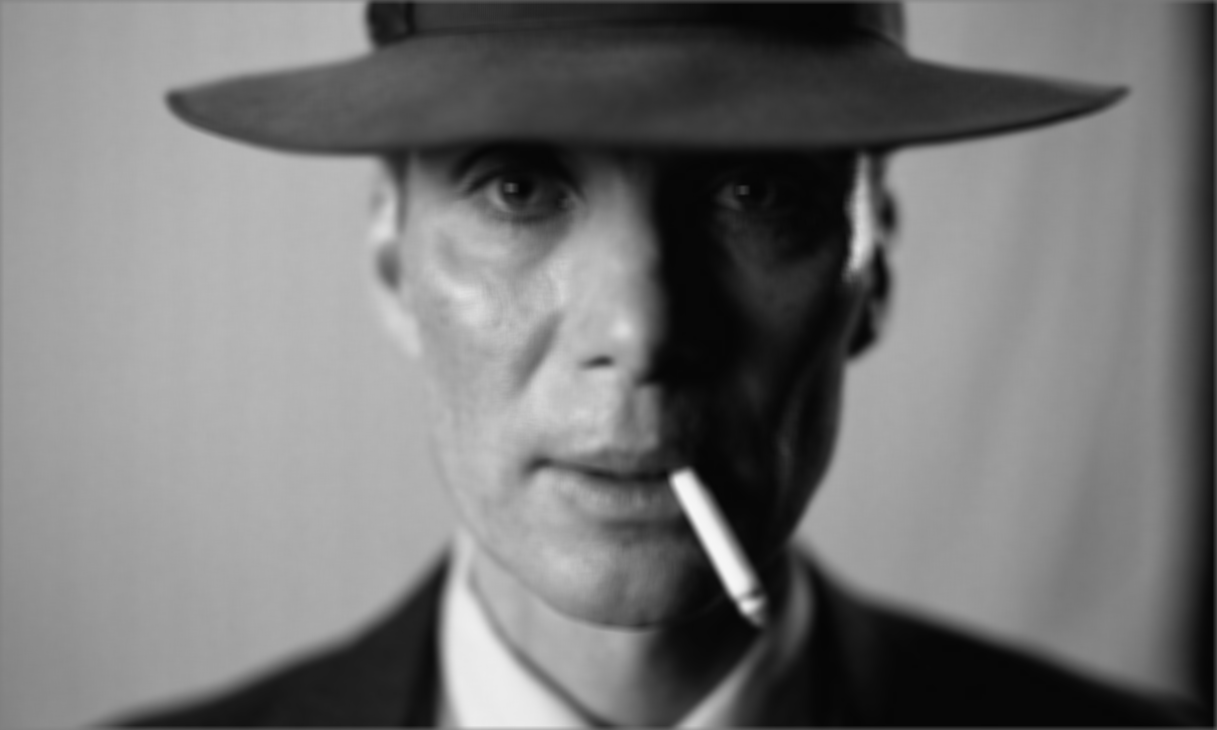
\includegraphics[width=0.45\textwidth]{result1//smooth_average_kernelSize=9.png}}
    \caption{smoothed figures by local average method with different kernel sizes}
\end{figure}

The smoothed figures by the Gauss kernel method are like:
\begin{figure}[H]
    \centering
    \subfigure[$\sigma$ = 1]
    {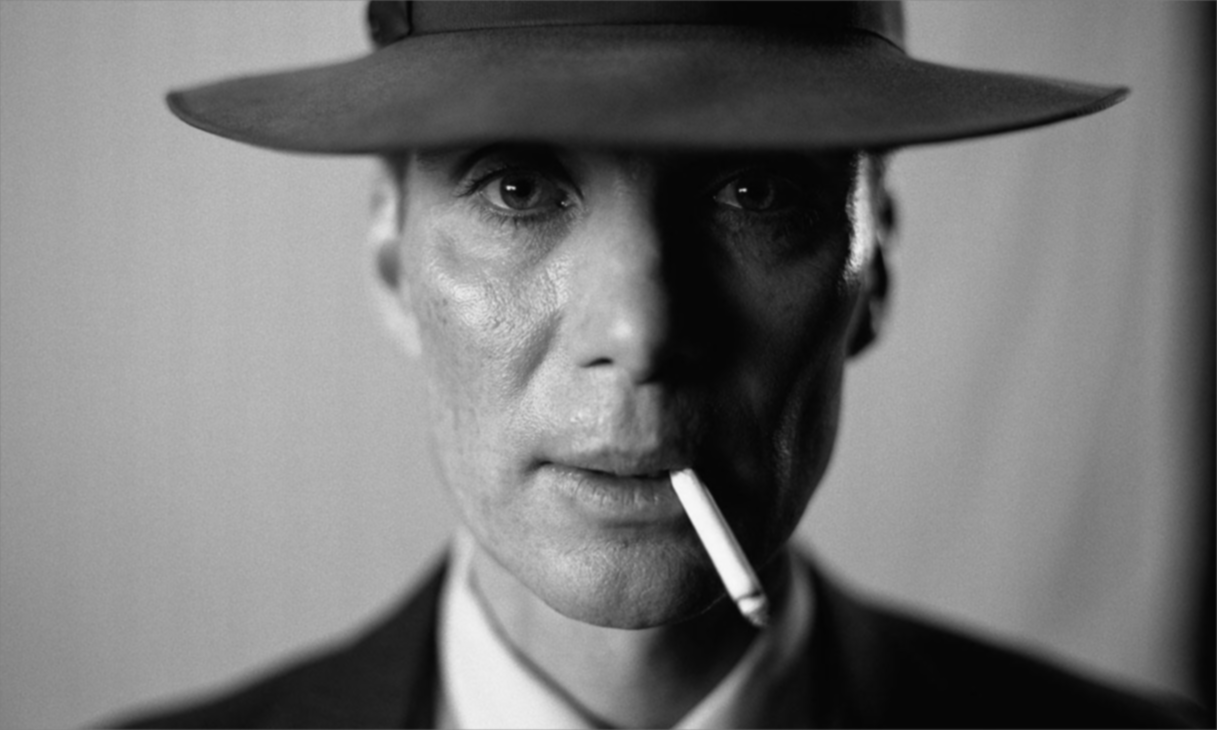
\includegraphics[width=0.45\textwidth]{result1//smooth_Gauss_sigma=1.png}}
    \,    
    \subfigure[$\sigma$ = 2]
    {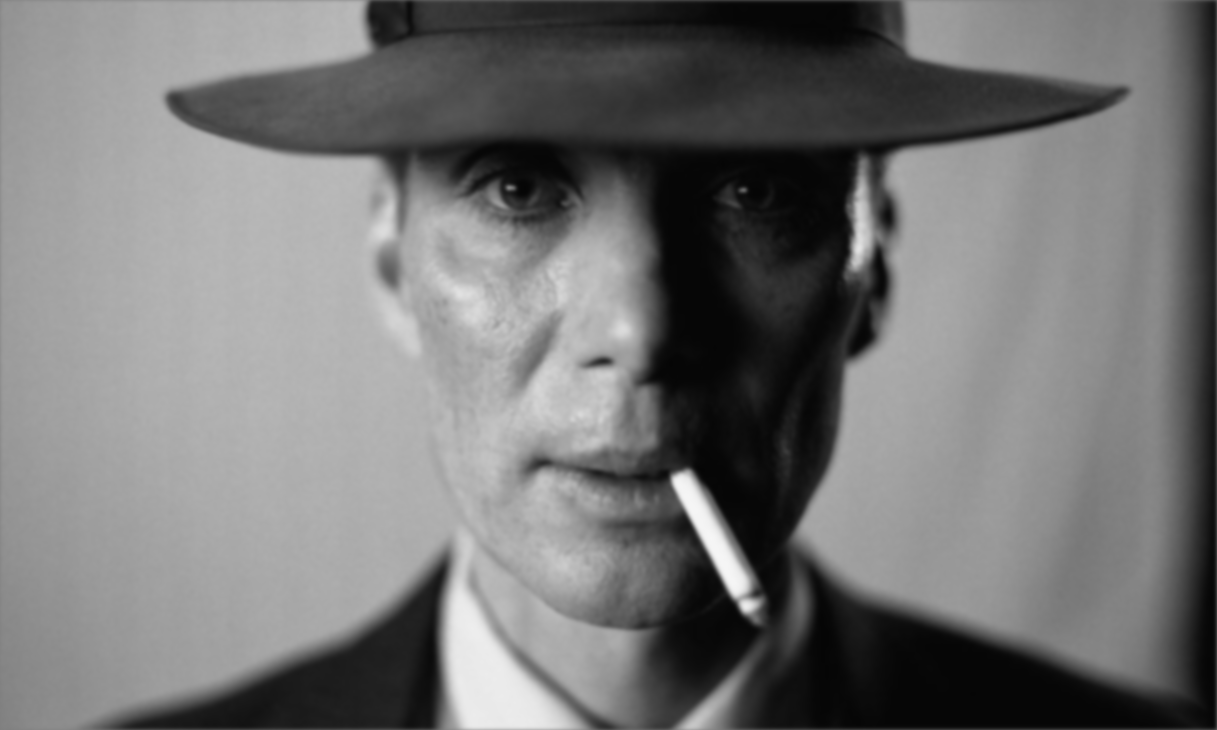
\includegraphics[width=0.45\textwidth]{result1//smooth_Gauss_sigma=2.png}}
    \,
    \subfigure[$\sigma$ = 3]
    {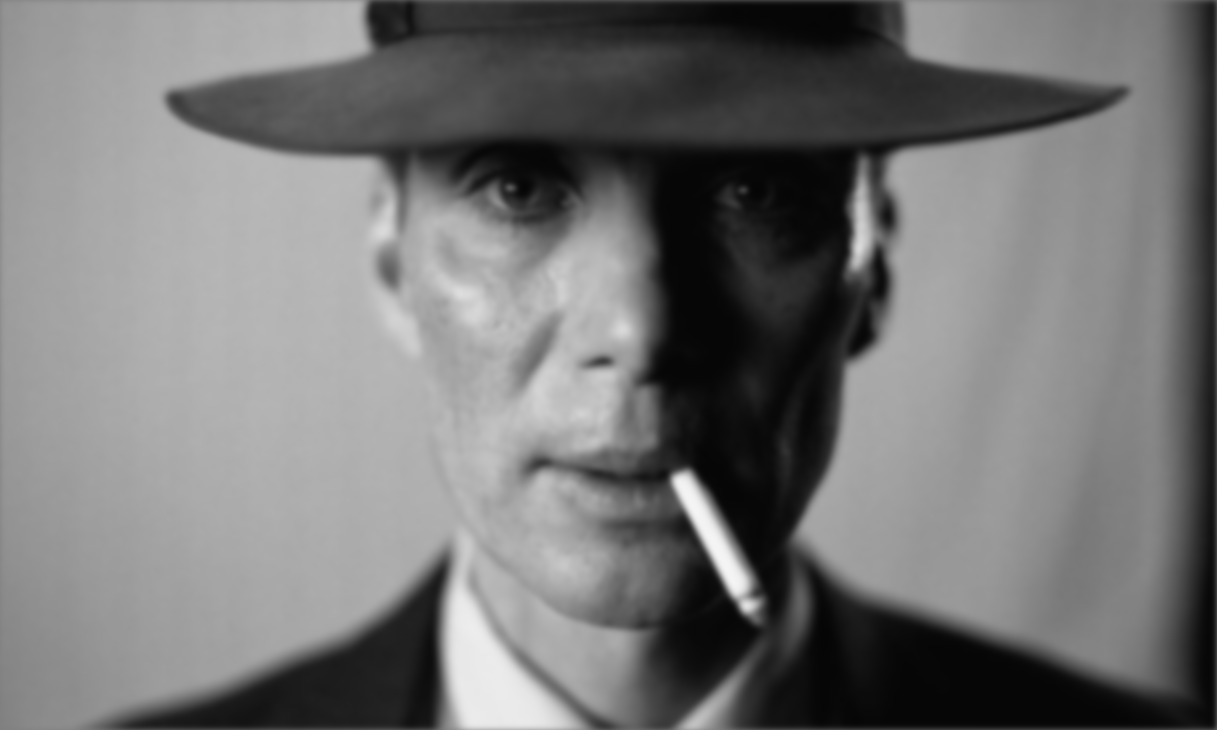
\includegraphics[width=0.45\textwidth]{result1//smooth_Gauss_sigma=3.png}}
    \,    
    \subfigure[$\sigma$ = 4]
    {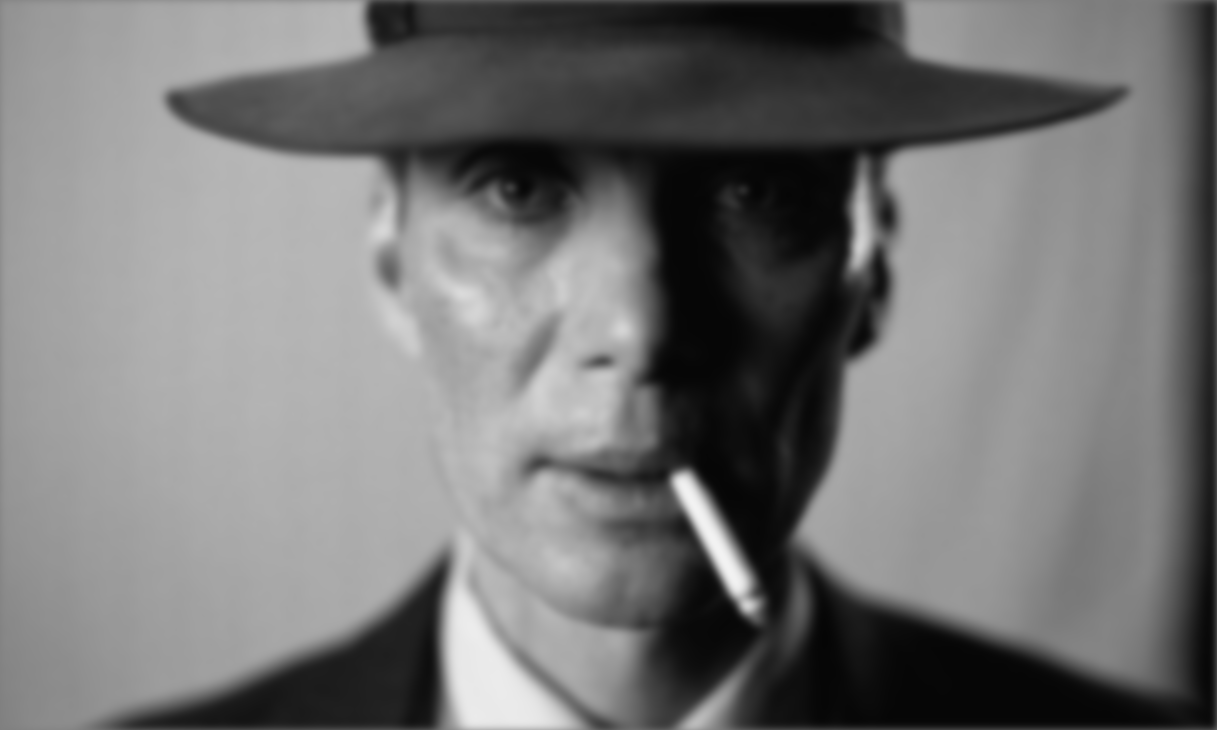
\includegraphics[width=0.45\textwidth]{result1//smooth_Gauss_sigma=4.png}}
    \caption{smoothed figures by Gauss kernel method with different $\sigma$}
\end{figure}

We can find the man's face are blurred after smoothing.

\subsection{Sharpening}
\subsubsection{Introduction to my Algorithm and Python Codes}
I also implement two methods for sharpening algorithm.
The first method is to make convolution with a \textbf{Laplacian operator}
and the second one is to add a \textbf{unsharp masking} to the original figure.

For the first method, users can set the coefficient $w$ in $g = (1+w\nabla^2)f$
and the algorithm will automatically check if the intensity after transform 
is still contained in $[0,255]$. The intensity larger than 255 will be set 255,
and the intensity less than 0 will be set 0.

For the second method, the algorithm first calculate the local average base on 
a Gauss Kernel with $\sigma=1$ and then get the unsharp musk. 
After that, add the unsharp musk to the original figure, i.e., 
$g = f + kh_{\text{mask}}$.
User can also 
set the coefficient $k$ for it and the algorithm will still
check and reset the intensity within $[0,255]$.

Similaryly, the algorithm will pad with pixels with intensity 127 before sharpening,
in order to keep the figure size.

Here are the python codes:
\lstinputlisting[style = Python,
caption={Python codes},
label = {sharp}]{exercise1_锐化.py} 

We take a picture of the surface of planet as the test figure. It is like:
\begin{figure}[H]
	\centering
	{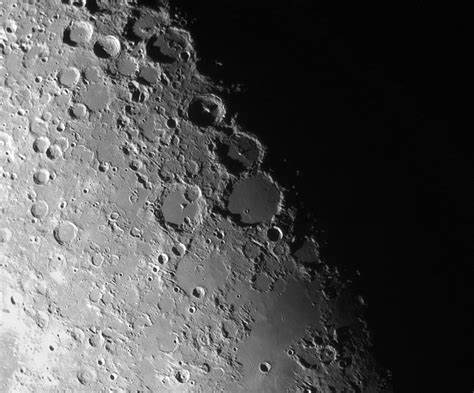
\includegraphics[width=0.45\textwidth]{test2.png}} 
	\caption{the original figure} \label{testFig2}
\end{figure}

And the results by Laplacian operator are as follows:
\begin{figure}[H]
    \centering
    \subfigure[$w$ = -20]
    {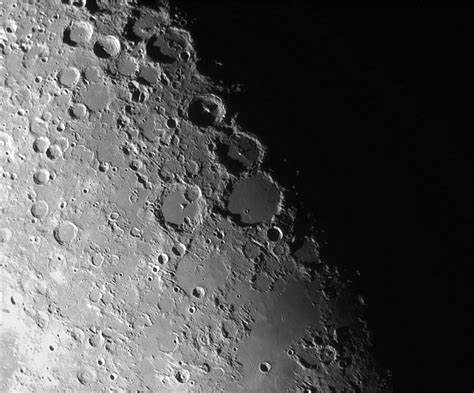
\includegraphics[width=0.45\textwidth]{result2//sharpen_Laplacian_w=-20.png}}
    \,    
    \subfigure[$w$ = -50]
    {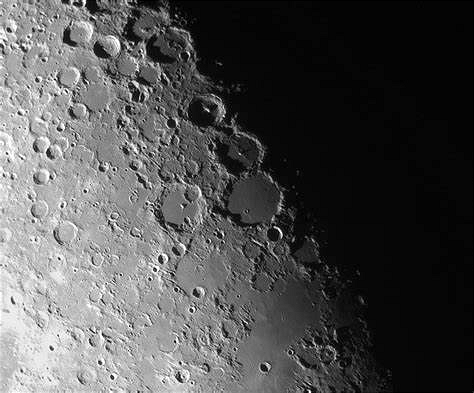
\includegraphics[width=0.45\textwidth]{result2//sharpen_Laplacian_w=-50.png}}
    \,
    \subfigure[$w$ = -80]
    {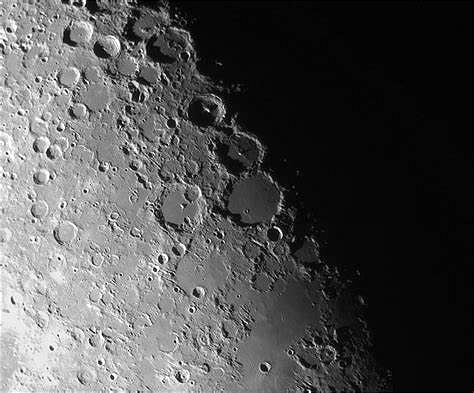
\includegraphics[width=0.45\textwidth]{result2//sharpen_Laplacian_w=-80.png}}
    \,    
    \subfigure[$w$ = -110]
    {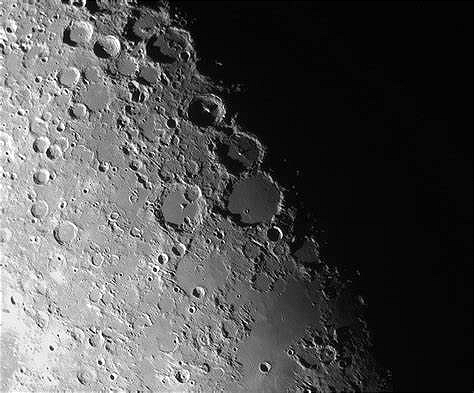
\includegraphics[width=0.45\textwidth]{result2//sharpen_Laplacian_w=-110.png}}
    \caption{sharpened figures by Laplacian operator method with different $w$}
\end{figure}

The results by adding unsharp musk are as follows:
\begin{figure}[H]
    \centering
    \subfigure[$k$ = 20]
    {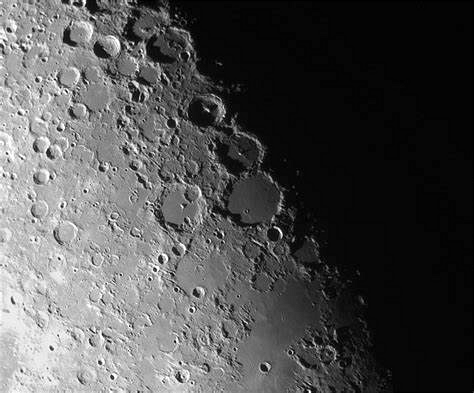
\includegraphics[width=0.45\textwidth]{result2//sharpen_highboost_sigma=1_k=20.png}}
    \,    
    \subfigure[$k$ = 50]
    {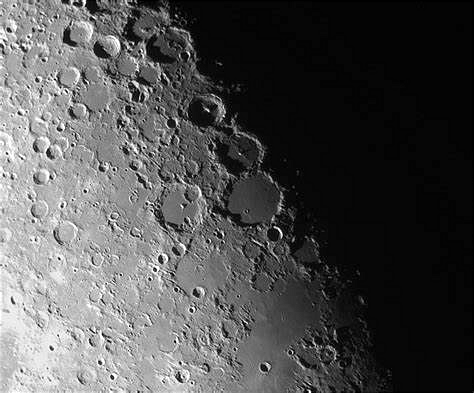
\includegraphics[width=0.45\textwidth]{result2//sharpen_highboost_sigma=1_k=50.png}}
    \,
    \subfigure[$k$ = 80]
    {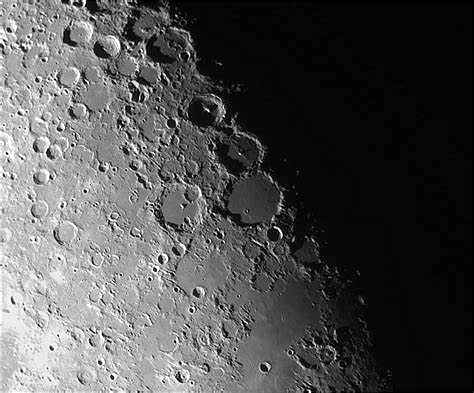
\includegraphics[width=0.45\textwidth]{result2//sharpen_highboost_sigma=1_k=80.png}}
    \,    
    \subfigure[$k$ = 110]
    {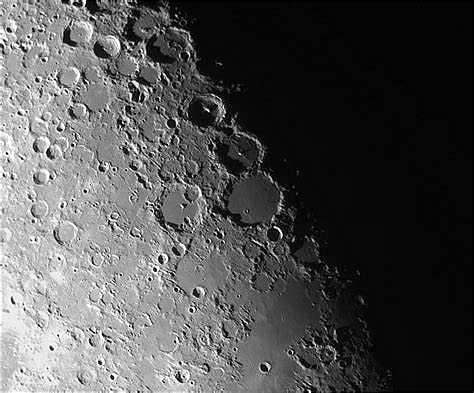
\includegraphics[width=0.45\textwidth]{result2//sharpen_highboost_sigma=1_k=110.png}}
    \caption{sharpened figures by adding unsharp musk with different $k$}
\end{figure}

We can find the sharpened figures show more details on the surface of the planet.

\section{Proofs about Frequence Transform}
\subsection{Impulse Train after Frequence Transform}
An impulse train is:
\[s_{\Delta T}(t) = \sum_{n=-\infty}^{\infty} \delta(t-n\Delta T) \]
We can re-write  $s_{\Delta T}(t)$ as Fourier series
\[ s_{\Delta T}(t) = \sum_{n=-\infty}^{\infty} c_n \text{e}^{j\frac{2\pi n}{\Delta T}t}  \]
where
\[c_n = \frac{1}{\Delta} \int_{-\Delta T/2}^{\Delta T/2} s_{\Delta T}(t) \text{e}^{-j\frac{2\pi n}{\Delta T}t}\,\text{d}t\]
Since only $\delta(t)$ is contained in $[-\Delta T/2, \Delta T/2]$, therefore
\begin{align*}
c_n &= \frac{1}{\Delta} \int_{-\Delta T/2}^{\Delta T/2} \delta(t) \text{e}^{-j\frac{2\pi n}{\Delta T}t}\,\text{d}t \\
&= \frac{1}{\Delta  T} \text{e}^0 \\
&= \frac{1}{\Delta T}
\end{align*}
Hence
\[s_{\Delta T}(t) = \frac{1}{\Delta T}\sum_{n=-\infty}^{\infty}  \text{e}^{j\frac{2\pi n}{\Delta T}t}\]

Now derive the Fourier transform of $\text{e}^{j\frac{2\pi n}{\Delta T}t}$. Since 
\begin{align*}
    \mathscr{F}^{-1} \left\{\ \delta(\mu-\mu_0) \right\} &= \int_{-\infty}^{\infty}\delta(\mu-\mu_0)\text{e}^{j2\pi\mu t}\, \text{d}\mu\\
    &= \text{e}^{j2\pi\mu_0 t}
\end{align*}
therefore, 
\begin{align*}
    \mathscr{F} \left\{  \text{e}^{j2\pi\mu_0 t} \right\} &= \delta(\mu-\mu_0) \\
    \mathscr{F} \left\{  \text{e}^{j\frac{2\pi n}{\Delta T} t} \right\} &= \delta(\mu-\frac{n}{\Delta T})
\end{align*}

Finally we can obtain the Fourier transform of an impulse series
\begin{align*}
	\mathscr{F} \left\{    s_{\Delta T}(t)   \right\} & = \mathscr{F} \left\{    \frac{1}{\Delta T}\sum_{n=-\infty}^{\infty}  \text{e}^{j\frac{2\pi n}{\Delta T}t}  \right\}  \\
	& = \frac{1}{\Delta T}\sum_{n=-\infty}^{\infty}\mathscr{F} \left\{      \text{e}^{j\frac{2\pi n}{\Delta T}t}  \right\}\\
	& = \frac{1}{\Delta T}  \sum_{n=-\infty}^{\infty} \delta(\mu-\frac{n}{\Delta T})
\end{align*}
	
\subsection{The Discrete Frequence Transform of a Real Signal}

Suppose $f(x)$ is a real function, hence \{$f_n$\} are also real.
the DFT of $f(x)$ is:
\[F(m) = \sum_{n=0}^{M-1} f_n\text{e}^{-j2\pi mn/M},\quad m=0,1,2,\dots,M-1\]
And
\begin{align*}
	F(-m) &= \sum_{n=0}^{M-1} f_n\text{e}^{j2\pi mn/M}  \\
\end{align*}
its conjucate is
\begin{align*}
\overline{F(-m)} &= \overline{\sum_{n=0}^{M-1} f_n\text{e}^{j2\pi mn/M} }=\sum_{n=0}^{M-1} f_n\text{e}^{-j2\pi mn/M} = F(m)
\end{align*}
Now we come to the conclusion that the DFT of real function  $f(x)$ is conjugate symmetric.

\subsection{The convolution theorem of 2-Dimension}
The proof of the convolution theorem of 2-dimension is as follows:
\begin{align*}
&\mathscr{F} \{ f(x,y) \ast h(x,y) \}(u,v)    \\
&= \mathscr{F}\left\{  \sum_{m=0}^{M-1}\sum_{n=0}^{N-1} f(m,n) h(x-m,y-n) \right\}(u,v) \\
&= \sum_{x=0}^{M-1} \sum_{y=0}^{N-1} \sum_{m=0}^{M-1} \sum_{n=0}^{N-1} f(m,n) h(x-m,y-n) \exp\left\{ -j2\pi\left(\frac{ux}{M}+\frac{vy}{N}\right)  \right\} \\
&=  \sum_{x=0}^{M-1} \sum_{y=0}^{N-1} \sum_{m=0}^{M-1} \sum_{n=0}^{N-1} f(m,n) h(x-m,y-n) \exp\left\{ -j2\pi\left(\frac{u(x-m)}{M}+\frac{v(y-n)}{N} + \frac{um}{M} + \frac{vn}{N}  \right)  \right\} \\
&=   \sum_{m=0}^{M-1} \sum_{n=0}^{N-1} \sum_{x=0}^{M-1} \sum_{y=0}^{N-1} f(m,n) h(x-m,y-n) \exp\left\{ -j2\pi\left(\frac{u(x-m)}{M}+\frac{v(y-n)}{N} + \frac{um}{M} + \frac{vn}{N}  \right)  \right\} \\
&  =    \sum_{m=0}^{M-1} \sum_{n=0}^{N-1} f(m,n)  \exp\left\{ -j2\pi\left( \frac{um}{M} + \frac{vn}{N}  \right)  \right\}   
			 \sum_{x=0}^{M-1} \sum_{y=0}^{N-1}  h(x-m,y-n)   \exp\left\{ -j2\pi\left(\frac{u(x-m)}{M}+\frac{v(y-n)}{N} \right)  \right\}
\end{align*}

\textbf{Since both $h(x,y)$ and $\exp\left\{ -j2\pi\left(\frac{u(x-m)}{M}+\frac{v(y-n)}{N} \right)  \right\}$
are periodic}, then we attain
\begin{align*}
	&\sum_{x=0}^{M-1} \sum_{y=0}^{N-1}  h(x-m,y-n)   \exp\left\{ -j2\pi\left(\frac{u(x-m)}{M}+\frac{v(y-n)}{N} \right)  \right\} \\
	&= \sum_{x=0}^{M-1} \sum_{y=0}^{N-1}  h(x,y)   \exp\left\{ -j2\pi\left(\frac{ux}{M}+\frac{vy}{N} \right)  \right\} \\
	&= \mathscr{F} \left\{h(x,y)\right\} (u,v)\\
	&= H(u,v)
\end{align*}
Therefore
\begin{align*}
	&\mathscr{F} \{ f(x,y) \ast h(x,y) \}(u,v) \\
	& =  \sum_{m=0}^{M-1} \sum_{n=0}^{N-1} f(m,n)  \exp\left\{ -j2\pi\left( \frac{um}{M} + \frac{vn}{N}  \right)  \right\}H(u,v) \\
	& = \mathscr{F}\left\{ f(m,n) \right\}(u,v) \cdot H(u,v) \\
	& = F(u,v)\cdot H(u,v)
\end{align*}


On the other hand
\begin{align*}
	&\mathscr{F}^{-1}\{F(u,v)\ast H(u,v)\}(x,y)\\
	&= \frac{1}{MN} \sum_{u=0}^{M-1} \sum_{v=0}^{N-1}\left\{F(u,v)\ast H(u,v)\right\} \exp\left\{j2\pi \left(\frac{ux}{M}+\frac{vy}{N}\right)\right\}\\
	&= \frac{1}{MN} \sum_{u=0}^{M-1} \sum_{v=0}^{N-1}\sum_{p=0}^{M-1} \sum_{q=0}^{N-1} F(p,q) H(u-p,v-q) \exp\left\{j2\pi \left(\frac{ux}{M}+\frac{vy}{N}\right)\right\}\\
	&= \frac{1}{MN} \sum_{u=0}^{M-1} \sum_{v=0}^{N-1}\sum_{p=0}^{M-1} \sum_{q=0}^{N-1} F(p,q) H(u-p,v-q) \exp\left\{j2\pi \left(\frac{(u-p)x}{M}+\frac{(v-q)y}{N}+\frac{px}{M}+\frac{qy}{N}\right)\right\}\\
	& = \frac{1}{MN} \sum_{p=0}^{M-1} \sum_{q=0}^{N-1} F(p,q)  \exp\left\{j2\pi \left(\frac{px}{M}+\frac{qy}{N}\right)\right\}  \sum_{u=0}^{M-1} \sum_{v=0}^{N-1}H(u-p,v-q) \exp\left\{j2\pi \left(\frac{(u-p)x}{M}+\frac{(v-q)y}{N}\right)\right\} \\
	& = \frac{1}{MN} \left[MNf(x,y)\right] \left[MNh(x,y)\right]\\
	& = MNf(x,y)\cdot h(x,y)
\end{align*}

Now we have completed the proof.
\end{document}

% \begin{figure}[H]
% 	\centering
% 	{\includegraphics[width=0.35\textwidth]{image//ignorance.png}} 
% 	\caption{}
% \end{figure}


% \lstinputlisting[style = Python,
% caption={Python codes},
% label = {efficient},
% linerange={110-125}]{exercise3.py} 


% \begin{figure}[H]
%     \centering
%     \subfigure[patch size = 11]
%     {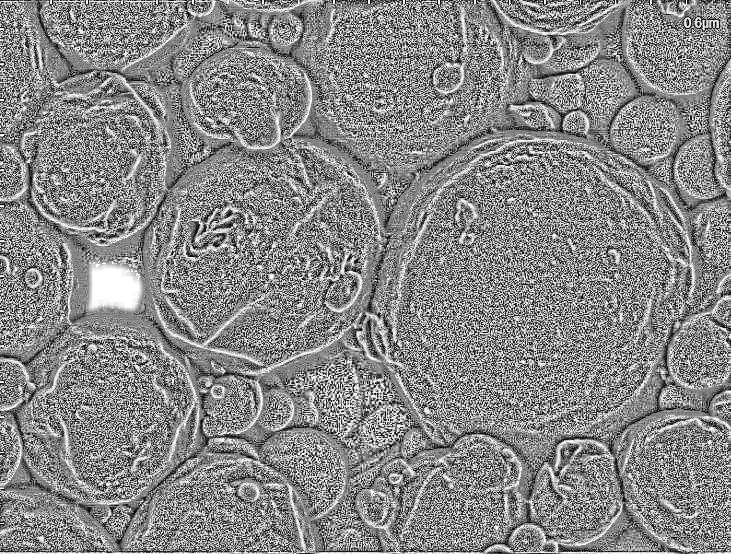
\includegraphics[width=0.49\textwidth]{image//local equalization with patch size = 11.jpg}}
%     \,    
%     \subfigure[patch size = 51]
%     {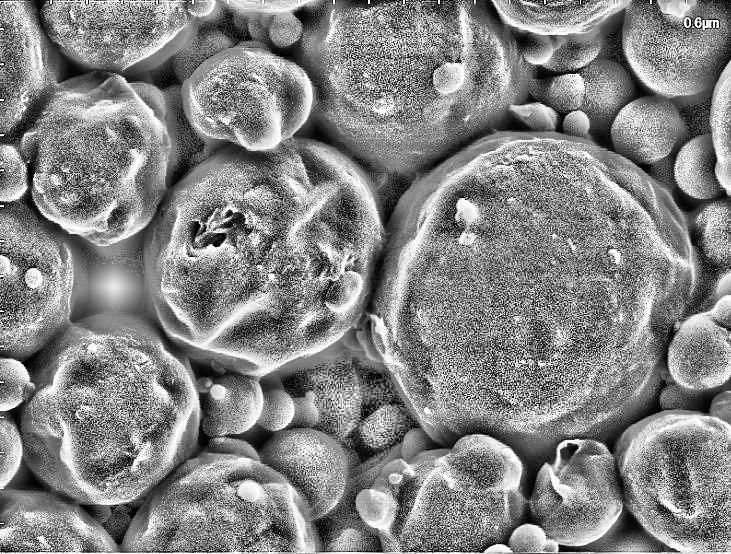
\includegraphics[width=0.49\textwidth]{image//local equalization with patch size = 51.jpg}}
%     \,
%     \subfigure[patch size = 151]
%     {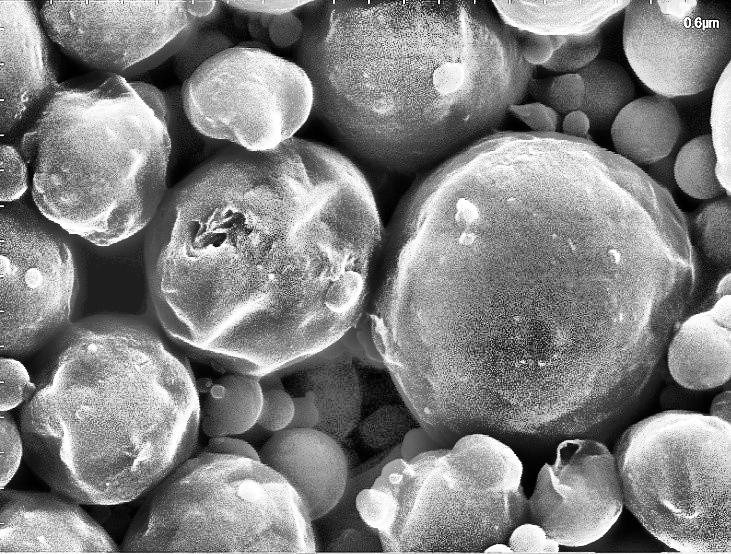
\includegraphics[width=0.49\textwidth]{image//local equalization with patch size = 151.jpg}}
%     \,    
%     \subfigure[patch size = 201]
%     {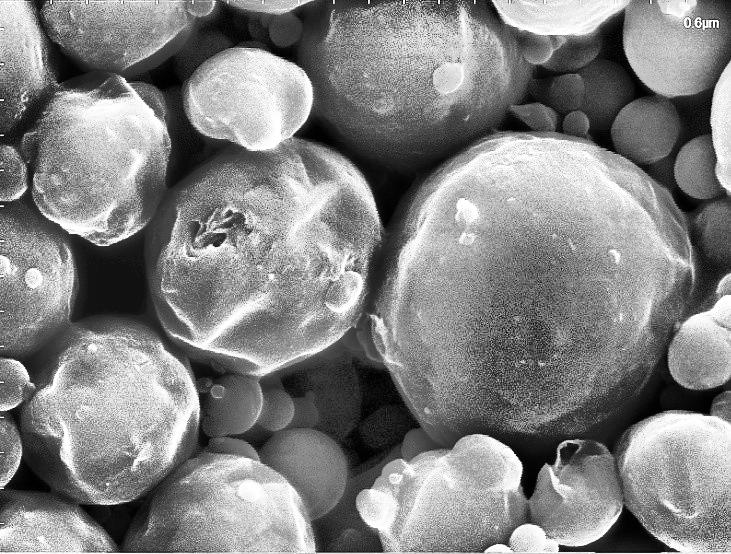
\includegraphics[width=0.49\textwidth]{image//local equalization with patch size = 201.jpg}}
%     \caption{local equalization with different patch sizes}
% \end{figure}
